\hypertarget{a-specific-project}{%
\subsection{A specific project}\label{a-specific-project}}

\hypertarget{motivation}{%
\subsubsection{Motivation}\label{motivation}}

This pattern can help project participants get started, get focused, and
make concrete change. It is especially useful for someone who is
currently feeling stuck.

\hypertarget{context}{%
\subsubsection{Context}\label{context}}

We often find ourselves confronted with what seems to be a difficult,
complex, or even insurmountable problem. It won't go away, but a
workable solution doesn't present itself, either. If there is a
candidate solution, it's also clear there are not enough resources for
it to be feasible.

\hypertarget{forces}{%
\subsubsection{Forces}\label{forces}}

\begin{quote}

\includegraphics{images/difficulty.png} \textbf{Difficulty}: bringing
about meaningful change is often hard work.\\

\includegraphics{images/inertia.png} \textbf{Inertia}: when things are
hard we may feel stuck, wring our hands, or preach to the choir.
\end{quote}

\hypertarget{problem}{%
\subsubsection{Problem}\label{problem}}

One is often blinded by one's prejudices and preferences. Some may put
considerable energy into pondering, discussing, exploring and feeling
stuck. Some may want more concrete progress, and notice the time passing
by. In a group setting, when the forward-movers ultimately try to act,
those who are more wrapped up in the experience of pondering and
exploring may rebel, if they feel that they are being left behind.
Inaction may seem like the only safe choice, but it has risks too. And,
once moving, things can easily get bogged down again.

\hypertarget{solution}{%
\subsubsection{Solution}\label{solution}}

One way to make progress when you're stuck is to ask a specific question
to someone who may be able to help you get unstuck. Formulating a
question helps your thinking become more concrete. Sometimes you'll see
that a solution was within your grasp all along. Often, one question
won't be enough, but you can repeat the process. In this way, you can
reduce a large, complex, or ephemeral concern into a collection of
smaller, specific, manageable tasks with clear next steps and success
criteria. Use a {{Scrapbook}} to make note of all the small things, and
weave them into your project {{Roadmap}}. This will show how the small
pieces relate to the bigger picture. If you have a fairly specific idea
about what you want to do, but you're finding it difficult to get it
done, don't just ask for advice: recruit material help (cf.~{{Carrying
capacity}}). One example of a specific project from the Peeragogy
project is our work on this paper, which had a specific target audience,
a set of associated deadlines, and allowed us to get help from pattern
experts.

\hypertarget{rationale}{%
\subsubsection{Rationale}\label{rationale}}

We've seen time and again that having a specific project is a recipe for
getting concrete, and that getting concrete is necessary for bringing
about change. Asking for help (which is what happens when you vocalize a
question) is one of the best ways to gain coherence. Making yourself
understood can go a long way toward resolving deeper difficulties.

\hypertarget{resolution}{%
\subsubsection{Resolution}\label{resolution}}

Where you run into \textbf{difficulty}, getting specific paves the way
for incremental forward progress and helps to overcome \textbf{inertia}.
The struggle between consensus and action is resolved in a tangible
project that combines action with dialog. Learning something new is a
strong sign that things are working. In the Peeragogy project, we have
completed many projects during our weekly hangouts, for example ``hive
editing'' an abstract for submission to a conference.

\hypertarget{example-1}{%
\subsubsection{Example 1}\label{example-1}}

At first glance, the Wikimedia Foundation's mission may seem like a good
idea, but hard to do anything about.\footnote{\url{https://wikimediafoundation.org/wiki/Mission_statement}}
practice, many Wikipedians contribute to the mission by working on {{A
specific project}}.

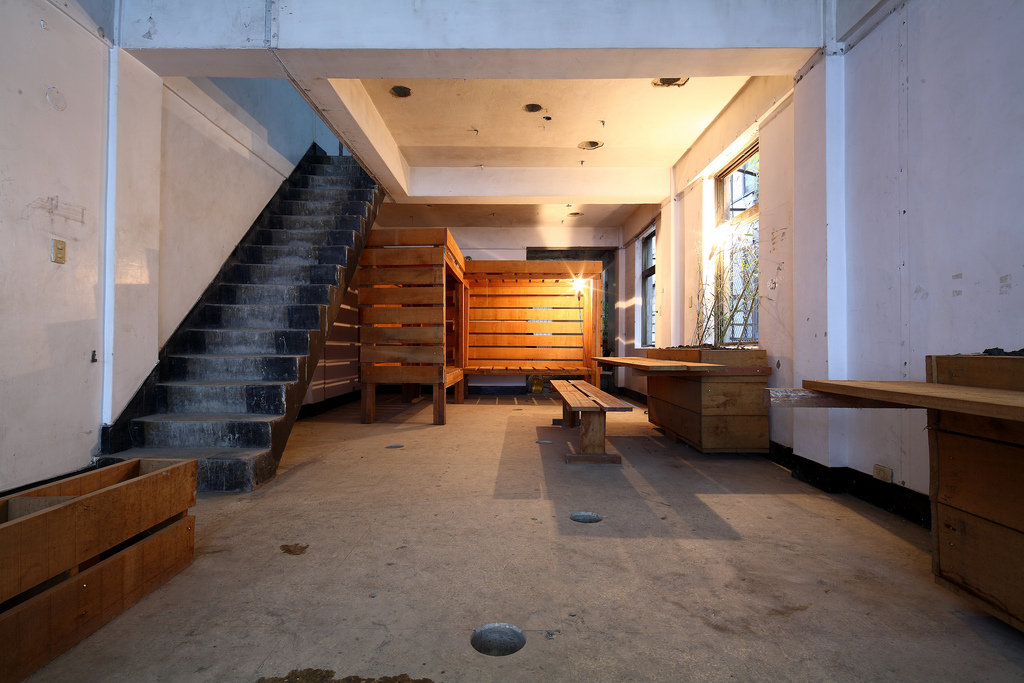
\includegraphics{images/Ruin_Academy_Dorm.jpg} \emph{Dormitory, Ruin
Academy, Taipei, Taiwan.}

Within Wikipedia, these are known as
``WikiProjects.''\footnote{\url{https://en.wikipedia.org/wiki/Wikipedia:WikiProject_Council/Directory}},\footnote{\^{}fn3}
on how to start new WikiProjects.\footnote{\url{https://en.wikipedia.org/wiki/Wikipedia:WikiProject_Council/Guide/WikiProject}}
Wikimedia Foundation also runs other public projects, including the
Wikipedia Education Program and the GLAM Wiki (for Galleries, Libraries,
Archives, and Museums).\footnote{\url{https://outreach.wikimedia.org/wiki/Education/Wikipedia_Education_Collaborative/Tasks}},\footnote{\url{https://outreach.wikimedia.org/wiki/GLAM}}
\emph{list of case studies that describes specific projects undertaken
by cultural organizations and Wikimedia}.\footnote{\url{https://outreach.wikimedia.org/wiki/GLAM/Case_studies}}

\hypertarget{example-2}{%
\subsubsection{Example 2}\label{example-2}}

Collegial and convivial peer support via remote collaboration or
short-term meet-ups may fill some of the requirements of ``student
life''. Peeragogy can also happen in neighborhoods, and among persons
sharing long-term co-habitation. While a traditional Dormitory may not
be necessary, a shared rented or cooperatively-owned living/working
environment could be an asset for peeragogues working together on {{A
specific project}}.

\hypertarget{whats-next-in-the-peeragogy-project}{%
\subsubsection{What's Next in the Peeragogy
Project}\label{whats-next-in-the-peeragogy-project}}

Let's use our pattern catalog to build specific, tangible ``what's
next'' steps, add them to our {{Roadmap}}, and carry them out with
concrete actions. Let's be sure we know who's responsible for what, and
employ a ``buddy system'' to help get things done.

\begin{center}\rule{0.5\linewidth}{0.5pt}\end{center}
